% !TeX root = Tutorial_13_Two-phase_flow.tex

\documentclass[a4paper, 14pt, twoside]{article}
\usepackage[14pt]{extsizes}
\usepackage[english,russian]{babel}
\usepackage[utf8]{inputenc}
\usepackage{amsfonts, amsmath, amssymb,amsthm, graphics,latexsym}
\usepackage{color}
\usepackage{wasysym}
\usepackage{misccorr}
\usepackage{mathrsfs}
\usepackage[active]{srcltx}
\usepackage{amsthm,fullpage}
\usepackage{fullpage}
\usepackage{multicol}
\usepackage[pdftex]{graphicx}
\usepackage[square, numbers]{natbib}
%\usepackage{fancyhrd}
%\usepackage{morefloats}
\usepackage{caption}
\usepackage{xcolor}
\usepackage{ifthen}
\usepackage{verbatim}
\usepackage{makeidx}
\usepackage{enumerate}
\usepackage{float}
\usepackage{graphicx,fancybox}
\usepackage{bm}
\usepackage{pdfcomment}
%\usepackage{indentfirst}
% \usepackage{commath}

\usepackage{hyperref} % For \url command

\usepackage{mathtools} % for def over equal sign command

\usepackage[makeroom,thicklines]{cancel} % For commands to cross-out math symbols. See http://tex.stackexchange.com/questions/75525/how-to-write-crossed-out-math-in-latex

\usepackage[left=3cm,right=2cm,
    top=3cm,bottom=3cm,bindingoffset=0cm]{geometry}
    
\usepackage{empheq} % for empheq environment
\usepackage{listingFreeFem}
\usepackage{appendix}

\lstset{
	columns=fullflexible,
	frame=shadowbox,
	numbers=left,
	numberstyle=\color{gray},
	breaklines=true,
	postbreak=\mbox{\textcolor{red}{$\hookrightarrow$}\space},
}



    
%\fontsize{14}{16pt}\selectfont \sloppy \allowdisplaybreaks
%%\renewcommand{\baselinestretch}{1.5}
%\sloppy


%%%%%%%%%%%%%%%%%% COLORS %%%%%%%%%%%%%%%%%%%%%%%%%%%%%
\renewcommand{\CancelColor}{\color{red}} % Color for canceling terms in expression

% Command for text highlighting
% Usegae:
%       \highlight{text}{color}
\newcommand{\highlight}[2]{
    \textbf{\color{#2}#1}}  % 

\newcommand{\todo}[1]{\textbf{\color{red}#1}}

%%%%%%%%%%%%%%%%%% MATH OPERATORS %%%%%%%%%%%%%%%%%%%%%%%%%%%%%
\DeclareMathOperator\dv{div} % divegence
\DeclareMathOperator\id{I}   % identity matrix
\DeclareMathOperator\tr{tr}  % trace operator
\DeclareMathOperator{\E}{E}  % Large strain tensor
\DeclareMathOperator{\const}{const} % const value 
\DeclareMathOperator{\rank}{rk}
%%%%%%%%%%%%%%%%%% BOLD SYMBOLS %%%%%%%%%%%%%%%%%%%%%%%%%%%%%
\newcommand{\bX}{\mathbf{X}}  % bold X
\newcommand{\bv}{\bm{v}}  % bold v
\newcommand{\bu}{\mathbf{u}}  % bold u
\newcommand{\bw}{\mathbf{w}}  % bold w
\newcommand{\bq}{\mathbf{q}}  % bold q
\newcommand{\bx}{\mathbf{x}}  % bold x
\newcommand{\be}{\mathbf{e}}  % bold e
\newcommand{\bs}{\mathbf{s}}  % bold s
\newcommand{\bn}{\mathbf{n}}  % bold n
\newcommand{\bp}{\mathbf{p}}  % bold p
\newcommand{\bff}{\mathbf{f}}  % bold f
\newcommand{\bc}{\mathbf{c}}  % bold c
\newcommand{\bbf}{\mathbf{f}}  % bold f
\newcommand{\bt}{\mathbf{t}} % bold T

\newcommand{\bD}{\mathbf{D}}  % bold D
\newcommand{\bP}{\mathbf{P}}  % bold P
\newcommand{\bcu}{\mathbf{U}} % bold U
\newcommand{\bct}{\mathbf{T}} % bold T

\newcommand{\bpsi}{\boldsymbol{\psi}} % bold psi
\newcommand{\bsigma}{\boldsymbol{\sigma}} % bold sigma
\newcommand{\btau}{\bm{\tau}} % bold tau
%%%%%%%%%%%%%%%%%% CALLIGRAPHIC SYMBOLS %%%%%%%%%%%%%%%%%%%%%%%%%%%%%
\newcommand{\epss}{{\cal E}}
\newcommand{\cL}{{\cal L}}
\newcommand{\cT}{{\cal T}}
\newcommand{\cQ}{{\cal Q}}

%%%%%%%%%%%%%%%%%% DIFFERENTIAL OPERATORS %%%%%%%%%%%%%%%%%%%%%%%%%%%%%
\newcommand{\pd}[2]{ % partial first derivative
   \dfrac{\partial #1}{\partial #2}
} 
\newcommand{\opd}[2]{ % ordinary first derivative
    \dfrac{\mathrm{d} #1}{\mathrm{d} #2}
}
\newcommand{\pddB}[2]{ % partial first derivative with function bordered by braces
    \dfrac{\partial }{\partial #2}\Bigl(#1\Bigr)
} 
\newcommand{\pdd}[3]{ % partial second mixed derivative
    \dfrac{\partial^2 #1}{\partial #2 \partial #3}
}

\newcommand{\pddfirst}[2]{ % partial second derivative with respect to one variable
    \frac{\partial^2 #1}{\partial {#2}^2}
}

%%%%%%%%%%%%%%%%%% NEW COMMANDS %%%%%%%%%%%%%%%%%%%%%%%%%%%%%
\newcommand\myeq{\stackrel{\mathclap{\footnotesize \mbox{def}}}{=}}

%%%%%%%%%%%%%%%%%% RENEW COMMANDS %%%%%%%%%%%%%%%%%%%%%%%%%%%%%
\renewcommand{\leq}{\leqslant} % Beautiful <=
\renewcommand{\geq}{\geqslant} % Beautiful >=

%%%%%%%%%%%%%%%%%% THEOREM STYLES %%%%%%%%%%%%%%%%%%%%%%%%%%%%%
\theoremstyle{definition}
\newtheorem{Lemma1}{Лемма}
\theoremstyle{definition}
\newtheorem{Problem}{Задача}
\newtheorem{Definition}{Определение}

\theoremstyle{remark}
\newtheorem*{Solution}{РЕШЕНИЕ}
\newtheorem*{Tip}{ПОДСКАЗКА}

%%%%%%%%%%%%%%%%%% PATHS TO FOLDERS WITH IMAGES %%%%%%%%%%%%%%%%%%%%%%%%%%%%%
\graphicspath{{img/}}

%%%%%%%%%%%%%%%%%% OTHER CUSTOMIZATIONS %%%%%%%%%%%%%%%%%%%%%%%%%%%%%
\everymath{\displaystyle} % Make all maths looks good

\DeclareMathOperator{\diver}{div}
\DeclareMathOperator\arctanh{arctanh}


%\textheight 240mm
%\textwidth 16cm
%\topmargin -15mm %было-15mm
%\multlinegap=0pt
\author{Калинин С.А., Кузнецов В.А., Стамлер К.В.}

%\title{Семинары по <<Введению в МСС>>}





%\makeatletter
%\newcommand*{\toccontents}{\@starttoc{toc}}
%\makeatother


\begin{document}

\title{Задача моделирования дфухфазной 2D фильтрации при наличии добывающей и нагнетательной скважины}
\maketitle

\newpage

\tableofcontents


\newpage


\section{Краткое описание решаемой задачи}

Требуется численно решить проблему двухфазной фильтрации воды и нефти в двумерной области при 
наличии добывающих и нагнетательных скважин. Для этого сначала записывается математическая 
формулировка задачи в дифференциальной и слабой постановке,
а далее используется пакет с открытым исходным кодом FreeFem++ \cite{MR3043640}. В качестве численного
метода во FreeFem++ используется метод конечных элементов.\\
В отличие от упрощенной задачи Баклея-Леверетта, где скорость по
всей расчетной области принималась постоянной, в данной работе учитывается 
наличие различного градиента давления, а значит и скорости, в различных точках области. Кроме того, в качестве
функций источника предполагается использовать точечные источники (соответствуют нагнетательным
вертикальным скважинам) и стоки (добывающие вертикальные скважины). Использование точечных 
источников немного меняет численную реализацию решения задачи и может вызывать дополнительные сложности в решении.

\section{Основные соотношения}

\subsection{Обозначения}

Здесь и далее жирными буквами обозначены векторные или тензорные величины. Ниже приведен список
используемых переменных и указана их размерность в СИ:\\
$S_w$~---~насыщенность водой [безразм.];\\
$\phi$~---~пористость [безразм.];\\
$\rho_w$~---~плотность воды [$\text{кг}/\text{м}^3$];\\
$\bm{v}_{rw}$~---~относительная скорость фильтрации воды в присутствии нефти;\\
$\bm{v}_{ro}$~---~относительная скорость фильтрации нефти в присутствии воды;\\
$q_w$~---~удельный (на мощность пласта, т.е. $[\text{м}^2/\text{с}]$) расход или поток воды;\\
$q_o$~---~удельный (на мощность пласта, т.е. $[\text{м}^2/\text{с}]$) расход или поток нефти;\\ 
$q_t$~---~удельный (на мощность пласта, т.е. $[\text{м}^2/\text{с}]$) полный расход флюида;\\
$Q_{inj}$~---~полный расход флюида на нагнетательную скважину $[\text{м}^3/\text{с}]$;\\
$Q_{prod}$~---~полный расход флюида на добывающую скважину $[\text{м}^3/\text{с}]$;\\
$K$~---~абсолютная проницаемость (в общем случае тензор) [$\text{м}^2$];\\
$k_{rw}$~---~относительная фазовая проницаемость по воде [безразм.];\\
$k_{ro}$~---~относительная фазовая проницаемость по нефти [безразм.];\\
$p_w$~---~давление в водной фазе [Па];\\
$p_o$~---~давление в нефтяной фазе [Па];\\
$\mu_w$~---~вязкость воды [Па*с];\\
$\mu_o$~---~вязкость нефти [Па*с];\\
$\nabla$~---~оператор градиента;\\
$\bm{n}$~---~вектор внешней нормали;\\
$\overline{\bm{q}}_\alpha$~---~заданный вектор потока флюида через границу, где $\alpha \in \{inj,prod\}$;\\
$R_\Omega$~---~невязка дифференциального уравнения внутри расчетной области;\\
$R_\Gamma$~---~невязка для граничного условия по границе расчетной области;\\
$\xi$~---~весовая функция для давления внутри расчетной области;\\
$\overline{\xi}$~---~весовая функция для давления на границе расчетной области;\\
$\psi$~---~весовая функция для водонасыщенности;\\
$L$~---~длина расчетной области [м];\\
$H$~---~ширина расчетной области [м].

\subsection{Дифференциальная постановка}

Уравнения двухфазного течения в породе включают в себя уравнения для переноса воды и нефти
\begin{equation}\label{eq:egor_common_equation_multiphase_rho}
\begin{split}
	\pd{(S_w \phi \rho_w)}{t} + \dv(\rho_w \bm{v}_{rw})    &=  \rho_w q_w, \quad \bm{v}_{rw}=-\frac{K k_{rw}}{\mu_w}\nabla p_w,\\
	\pd{(S_o \phi \rho_o)}{t} + \dv(\rho_o \bm{v}_{ro})  &=  \rhoы_o q_o, \quad \bm{v}_{ro}=-\frac{K k_{ro}}{\mu_o}\nabla p_o.
\end{split}
\end{equation}

$$
\rho_\alpha(p_\alpha) = \frac{\rho^{st}_\alpha}{B_\alpha}, \quad \alpha = w,o,
$$
где $\rho^{st}_\alpha,$~$B_\alpha$~---~плотности фильтрующихся жидкостей при некоторых стандартных (референсных) условиях и  коэффициенты объемного расширения соответственно. 
Здесь неявно полагается, что $B_\alpha$ является функцией давления.
Тогда сжимаемости воды и нефти примут вид 
\begin{equation}\label{eq:sibin_c_alpha}
c_\alpha = \frac{1}{\rho_\alpha} \pd{\rho_\alpha}{p_\alpha} = B_\alpha \pd{(1 / B_\alpha)}{p_\alpha}, \quad \alpha = w,o.
\end{equation}

Введем масштабированную насыщенность
\begin{equation}\label{eq:star:mod:Sw}
 \overline {S}_w= \frac{S_w-S_w^{cr}}{1-S_w^{cr}-S_o^{cr}},
\end{equation}
где $S_w^{cr}$ --- критическая водонасыщенность, при которой перестает течь вода, $S_o^{cr}$ --- критическая нефтенасыщенность, при которой перестает течь нефть. Тогда относительные фазовые проницаемости можно записать в следующем виде:
\begin{equation}\label{eq:star:mod:RelatPerm}
	k_{rw}= \begin{cases}
	0, \quad \text{при}\quad \overline {S}_w \leq 0,\\
	k_{rw}^0 (\overline {S}_w)^{n_w}, \,\text{при}\,0<\overline {S}_w <1, \\
	k_{rw}^0, \text{при}\quad \overline {S}_w \geq 1.
   \end{cases}
   k_{ro}=\begin{cases}
	k_{ro}^0, \quad \text{при}\quad \overline {S}_w \leq 0, \\
	k_{ro}^0 (1-\overline {S}_w)^{n_o}, \, \text{при}\,0<\overline {S}_w<1 , \\
   0, \quad \text{если}\quad \overline {S}_w \geq 1.\\
   \end{cases}
\end{equation}

\begin{figure}[H]
	\centering
	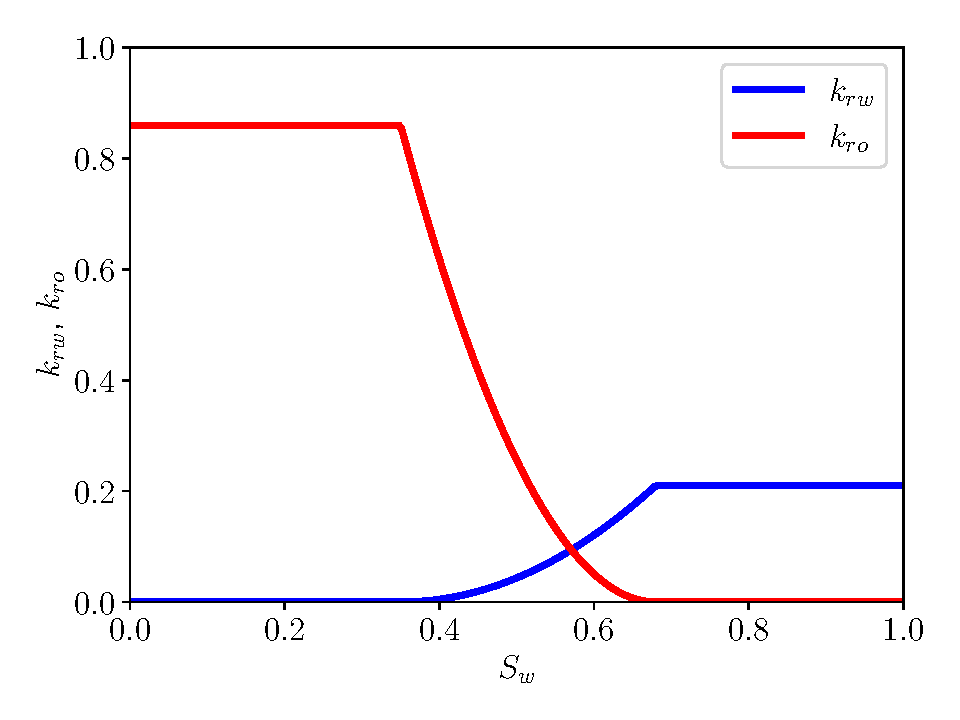
\includegraphics[width=0.7\linewidth]{img/RPP_Corey}
	\caption{Кривые ОФП по модели Кори}
	\label{fig:RPP_Corey}
\end{figure}

\subsubsection{Упрощающие предположения}
Будем считать, что коэффициеты объемного расширения постоянны в рассматриваемом диапазоне давлений и равны $B_\alpha = 1$, $\alpha = w,o$. Также пренебрежем влиянием капилярных сил:
\begin{equation}\label{eq:common_eq_capillar}
	p_c(S_w) = p_o - p_w = 0,
\end{equation}
что влечет равенство давлений в фазах.
Для насыщенностей фаз имеется соотношение
\begin{equation}\label{eq:So_Sw_1}
	S_o + S_w = 1.
\end{equation}
Предположим, что поровое пространство слабосжимаемое. Тогда
\begin{equation}\label{eq:compress_phi}
	c_r = \frac{1}{\phi} \pd{\phi}{p}, \quad p = p_w=p_o,
\end{equation}
при этом сама пористость приближенно считается постоянной $\phi=\phi_0$.

\subsubsection{Формулировка в переменных $p$---$S_w$}

Складывая уравнения с учетом упрощающих предположений, получим

\begin{equation}
    c_t\phi \pd{p}{t}
    + \dv\, \left( -\left(\frac{K k_{rw}}{\mu_w } +
     \frac{K k_{ro}}{\mu_o}\right)\nabla p \right) = q_w + q_o,
\end{equation}
Здесь полная сжимаемость $c_t$ определяется как:
\begin{equation}\label{eq:totalCompress}
	c_t= c_r + c_w  S_w + c_o (1-S_w)
\end{equation}
где~---~ $c_r$, $c_w$, $c_o$ сжимаемости пор  воды и нефти соответственно.
Уравнение на насыщенность воды запишется в виде (см. \ref{transport_eq_sub})
\begin{equation}\label{eq:star_common_equation_multiphase_satur}
	  \phi \pd{S_w}{t} + S_w\phi^0\left(c_r + c_w \right)\pd{p}{t} + \dv\, \left( -\frac{K k_{rw}}{\mu_w}\nabla p \right) = 
	  q_w.
\end{equation}

Заметим, что если ввести обозначения
\begin{equation}
    \bq_w = -K\frac{k_{rw}(S_w)}{\mu_w}\nabla p = -K \lambda_w(S_w) \nabla p,
\end{equation}
\begin{equation}
	\bq_o = -K\frac{k_{ro}(S_w)}{\mu_o}\nabla p = -K \lambda_o(S_w) \nabla p,
\end{equation}
то полный фильтрационный поток жидкости выражается в виде
\begin{equation}
    \bq_t = \bq_w + \bq_o = -K (\lambda_w(S_w) + \lambda_o(S_w)) \nabla p = -K (\lambda_t(S_w)) \nabla p,
\end{equation}
а фильтрационный поток воды можно записать как 
\begin{equation}
    \bq_w = f_w \bq_t, \quad f_w  = \dfrac{\lambda_w(S_w)}{\lambda_t(S_w)},
\end{equation}
где $f_w$ --- функция Баклея~---~Леверетта.

В этих терминах основные уравнения записываются в следующем виде:
\begin{equation}\label{eq:diffusion}
    c_t\phi \pd{p}{t}
    + \dv\, \left( \bq_t \right) = q_w + q_o, \quad \bq_t = - K \lambda_t \nabla p,
\end{equation}



\begin{equation}\label{eq:satur}
	\phi \pd{S_w}{t} + S_w\phi\left(c_r + c_w \right)\pd{p}{t} + \dv\, \left( f_w \bq_t \right) = 
	q_w.
\end{equation}
В общем случае также необходимо решить уравнение на эволюцию пористости
\begin{equation}\label{eq:porosity_evolution}
	\pd{\phi}{t} = \pd{\phi}{p} \pd{p}{t}  = c_r \phi \pd{p}{t}.
\end{equation}

\subsubsection{Задача вытеснения нефти водой в пятиточечном шаблоне заводнения}

Рассмотрим классическую задачу о вытеснении нефти водой для пятиточечного
шаблона заводнения. 
Предположим, что нам задана прямоугольная область $\Omega$ (рисунок~\ref{fig:ProblemInitBoundary}), 
внутри которой выполняются уравнения двухфазной фильтрации. 
\begin{figure}[H]
	\centering
	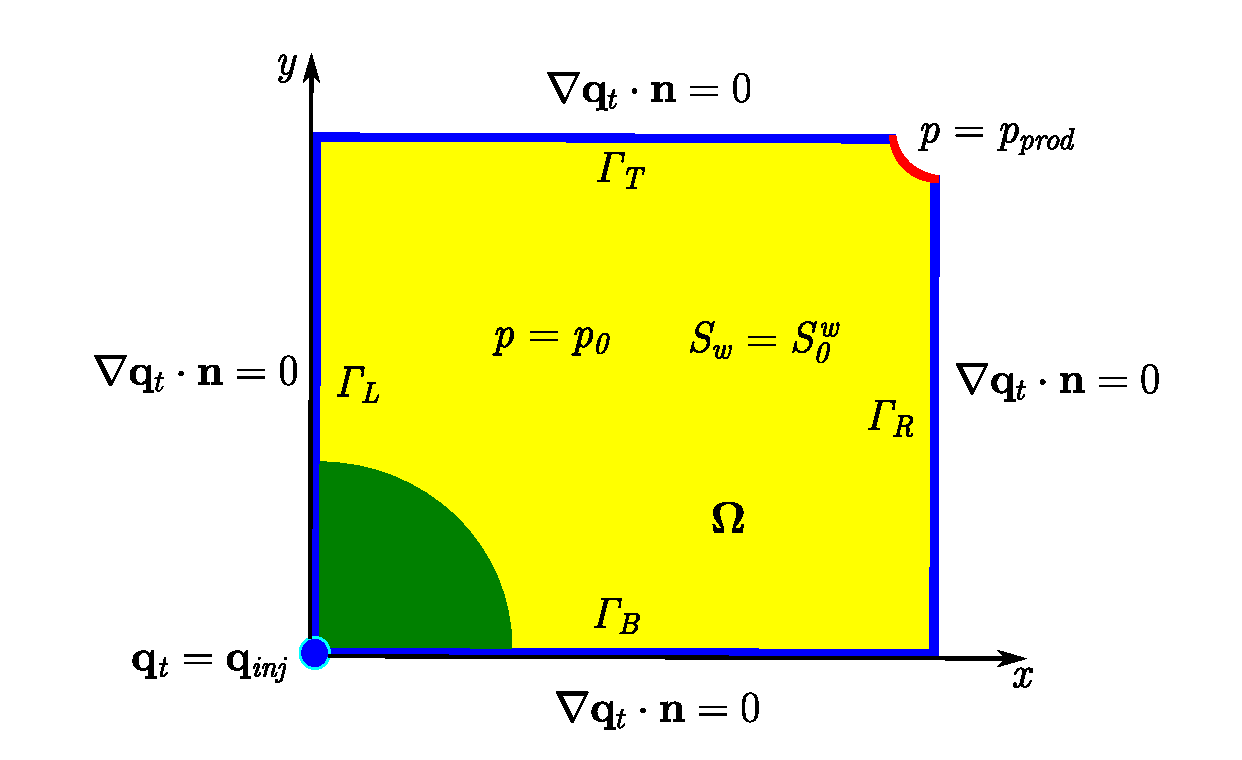
\includegraphics[width=1\linewidth]{img/Picture.pdf}
	\caption{Постановка задачи о вытеснении нефти водой для пятиточечного шаблона заводнения}
	\label{fig:ProblemInitBoundary}
\end{figure}

В силу симметрии задачи поток через все границы отсутствует, поэтому достаточно записать
\begin{equation}
	\Gamma_L, \Gamma_R, \Gamma_T, \Gamma_B: \quad \bq_t \cdot \bn = 0,
\end{equation}

Через левый нижний узел прямоугольной области производится закачка воды с заданным 
расходом и насыщенностью:
\begin{equation}\label{eq:GammaL}
	\Gamma_{inj}: \bm{q}_{t} = \overline{\bm{q}}_{inj}, \quad S_w = S_w^{inj}.
\end{equation}
Для практических целей интересно рассмотреть два типа граничных условий на добывающей скважине:\\
~---~задан известный поток;\\
~---~задано известное давление.\\
В первом случае расчетную область можно рассматривать как строго прямоугольную и в верхнем правом узле
задать поток в виде:
\begin{equation}\label{eq:GammaR}
	\Gamma_{prod}: \bm{q}_{t} = \overline{\bm{q}}_{prod}.
\end{equation}
Во втором случае необходимо изменить форму расчетной области и учесть конечные размеры скважины 
(радиус скважины), поскольку задание фиксированного давления в узле будет приводить к 
некорректной оценке дебита скважины. Если обозначить границу в верхнем правом узле как $\Gamma_{prod}$,
то можно записать граничные условия вида \refeq{eq:GammaR} как для случая одного узла, так и для 
конкретной геометрии скважины (красная граница на рисунке~\ref{fig:ProblemInitBoundary}).\\
В качестве начальных данных задаются следующие величины:
\begin{equation}\label{eq:init_cond}
	\Omega: \quad S_w\left|_{t=0} = S_w^0\right., \quad p\left|_{t=0} = p_0\right.  \quad \phi\left|_{t=0} = \phi_0\right..
\end{equation}



\subsection{Слабая постановка}


\subsubsection{Уравнение фильтрации}
Для получения слабой формулировки воспользуемся общим алгоритмом метода взвешенных невязок 
(\cite{Zenkevich_1986} стр.59 ур.(2.41)). В общем случае полагается, что системы весовых
функций для области $\Omega$ и границы $\Gamma$ отличаются и требуется приравнять нулю 
взвешенную сумму невязок внутри области и на границе, тогда
 \begin{equation}\label{eq:residuals}
	\int\limits_\Omega \xi R_\Omega \,d\Omega + \int\limits_\Gamma \overline{\xi}R_\Gamma \,d\Gamma = 0
 \end{equation} 
Поскольку внутри расчетной области $\Omega$ отсутствуют источники и стоки для фильтрующихся фаз,
то в уравнении на давлениие \refeq{eq:diffusion} правая часть равна нулю. В этом случае выражения для невязок 
по области и по границе примут следующий вид:
\begin{equation}
	\begin{aligned}
		R_\Omega &= c_t\phi \pd{p}{t} + \dv\, \left( \bq_t \right)\\
		R_\Gamma &= \bq_t - \overline{\bm{q}}_{\alpha}
	\end{aligned}
\end{equation}
 %В качестве тестовой функции для давления выберем $\xi$, при этом 
%\begin{equation}
%	\xi\left|_{\Gamma_L}\right. = 0.
%\end{equation}

Тогда уравнение \refeq{eq:residuals} перепишется как:

\begin{equation}
	\displaystyle 0=\int\limits_\Omega  (c_t\phi \pd{p}{t} + \dv{\bq_t}) \,\xi \,dx dy
	+ \int\limits_{\Gamma} (\bq_t - \overline{\bm{q}}_{\alpha})\cdot \bn \, \overline{\xi} \,ds
\end{equation}
В силу известного произвола в выборе системы весовых функций в полученном выражении примем, что
\begin{equation}
	\overline{\xi} = -\xi.
\end{equation}
Тогда, если применить теорему Грина (интегрирование по частям), то можно ослабить требования к гладкости
искомой функции и получить т.н. "слабую формулировку" для уравнения  диффузии 

\begin{multline}
	\displaystyle 0=\int\limits_\Omega c_t\phi \pd{p}{t}\, \xi \,dx dy 
	 + \int\limits_\Omega \dv{\bq_t}\, \xi \,dx dy
	 - \int\limits_{\Gamma} \bq_t\cdot \bn \, \xi \,ds 
	 + \int\limits_{\Gamma} \overline{\bm{q}}_{\alpha}\cdot \bn \, \xi \,ds = \\ 
	 \int\limits_\Omega c_t\phi \pd{p}{t}\, \xi \,dx dy 
	 + \int\limits_\Omega K \lambda_t \nabla p \cdot \nabla\xi \,dx dy \\
	 +\int\limits_{\Gamma_L} (\bq_t \cdot \bn) \xi \, ds
	 +\int\limits_{\Gamma_T\cup \Gamma_B} (\bq_t \cdot \bn) \xi \, ds
	 +\int\limits_{\Gamma_R} (\bq_t \cdot \bn) \xi \, ds \\
	 -\int\limits_{\Gamma_L} (\bq_t \cdot \bn) \xi \, ds
	 -\int\limits_{\Gamma_T\cup \Gamma_B} (\bq_t \cdot \bn) \xi \, ds
	 -\int\limits_{\Gamma_R} (\bq_t \cdot \bn) \xi \, ds 
	 +\int\limits_{\Gamma_{inj}\cup \Gamma_{prod}} \overline{\bm{q}}_{\alpha}\cdot \bn \, \xi \, ds\\ 
\end{multline}
Значения $\overline{\bm{q}}_{\alpha}$ всюду равны нулю на границе, кроме отдельных узлов (нижний левый и верхний правый узлы), а интегралы, содержащие $(\bq_t \cdot \bn)$ всегда сократятся
при условии $\overline{\xi} = -\xi$, поэтому окончательно для уравнения фильтрации получим

\begin{equation}\label{eq:PressureNeuman}
	0=\int\limits_\Omega c_t\phi \pd{p}{t}\, \xi \,dx dy 
	+ \int\limits_\Omega K \lambda_t \nabla p \cdot \nabla\xi \,dx dy - \frac{1}{4}Q_{inj}\, \xi(0,0)
	+ \frac{1}{4}Q_{prod}\, \xi(L,H)
\end{equation}
Здесь полагается, что интеграл по границе $\Gamma_{inj}\cup \Gamma_{prod}$ от $\overline{\bm{q}}_{\alpha}$ 
при стремлении диаметра скважины к нулю должен давать одну четверть от полного дебита скважины в силу симметрии.
Следует отметить, что уравнение \refeq{eq:PressureNeuman} может давать нефизичные решения с 
отрицательными давлениями где-то во внутренних точках области или на границе, поэтому нужно
поддерживать определенное соотношение между объемами закачиваемой и добываемой жидкости.
В случае, если решается задача с контролем по давлению на добывающей скважине следует переписать
слабую формулировку в следующем виде:

\begin{equation}\label{eq:PressureDirichlet}
	0=\int\limits_\Omega c_t\phi \pd{p}{t}\, \xi \,dx dy 
	+ \int\limits_\Omega K \lambda_t \nabla p \cdot \nabla\xi \,dx dy - \frac{1}{4}Q_{inj}\, \xi(0,0)
\end{equation}
Граничные условия Дирихле не записываются явно в слабой формулировке \refeq{eq:PressureDirichlet}  по причине того, что
значения искомой функции явно заданы в граничных узлах и их определения не требуется. На уровне матриц
происходит вычеркивание соответствующих строк и столбцов, с учетом известных значений в правых
частях матричных уравнений. Однако можно всегда формально отнести граничные значения искомой функции (на границе 
с условиями Дирихле) к неизвестным. В этом случае используется метод штрафных функций, который
интегрирован во FreeFem++ как оператор $\mathbf{on}$. 

\subsubsection{Уравнение переноса водонасыщенности}\label{transport_eq_sub}
Для вывода уравнения на насыщенность рассмотрим первое уравнение системы \ref{eq:egor_common_equation_multiphase_rho}.
Воспользуемся правилом производной произведения для слагаемого с производной по времени
\begin{equation}\label{eq:chain_rule}
\pd{(S_w \phi \rho_w)}{t}=\phi \rho_w \pd{S_w}{t}+S_w \rho_w \pd{\phi}{t}+S_w \phi \pd{\rho_w}{t}
\end{equation}
По определению, изотермическая сжимаемость фазы $l$ задается как
\begin{equation}\label{eq:isothermal_compressibility}
c_l=\frac{1}{\rho_l}\pd{\rho_l}{p} |_{T}
\end{equation}
Зависимость пористости от давления обычно задается в виде линейной функции:
\begin{equation}\label{eq:porosity_vs_p}
\phi = \phi^0 [1+c_r (p-p^0)],
\end{equation}
где $p^0$ ~---~ опорное давление, при котором определена пористость $\phi^0$.
В качестве опорного давления выбирается либо атмосферное давление, либо среднее
пластовое давление на данном месторождении.\\
Правило производной сложной функции пористости $\phi=\phi(p)$ задается выражением
\begin{equation}\label{eq:derivative_phi}
\pd{\phi}{t}=\pd{\phi}{p} \pd{p}{t}.
\end{equation}
Зависимость плотности от давления для слабосжимаемой жидкости
\begin{equation}\label{eq_rho_vs_p}
\rho_l=\rho^0_l[1+c_l(p-p^0)].
\end{equation}
Объемный коэффициент фазы $l$ (связанный с плотностью фазы) задается как 
\begin{equation}\label{eq:FVF}
B_l=\frac{\rho_{lsc}}{\rho_l}=\frac{B^0_l}{1+c_l(p-p^0)},
\end{equation}
причем $sc$ - standard conditions.\\
Правило производной сложной функции плотноти $\rho=\rho(p)$ определяется как
\begin{equation}\label{eq:derivative_rho}
\pd{\rho}{t}=\pd{\rho}{p} \pd{p}{t}.
\end{equation}
Подставляя в уравнение \ref{eq:chain_rule} выражения \ref{eq:porosity_vs_p}, \ref{eq:derivative_phi},\ref{eq_rho_vs_p}, \ref{eq:derivative_rho} и 
поделив на $\rho_w$ получим
\begin{multline}\label{eq:ext_chain_rule}
\pd{(S_w \phi \rho_w)}{t}=\phi \pd{S_w}{t}+ S_w \phi^0 c_r \pd{p}{t}+ S_w \phi c_w \pd{p}{t} = \\
\phi \pd{S_w}{t}+S_w(\phi^0 c_r + \phi^0 c_w + c_w c_r \phi^0 (p-p^0))\pd{p}{t}
\end{multline}
Если учесть, что $c_w c_r \rightarrow 0$

\begin{equation}\label{eq:approx_time_deriv}
\pd{(S_w \phi \rho_w)}{t} \approx \phi \pd{S_w}{t}+S_w \phi^0 (c_r+c_w)\pd{p}{t}
\end{equation}
Если применить стандартный прием метода конечных элементов к исходному уравнению на водонасыщенность, то известно, 
что получится неустойчивая разностная схема.
Поэтому к исходному уравнению на водонасыщенность добавим член с искусственной диффузией. 
С физической точки зрения данное слагаемое появляется из-за присуствия капиллярных сил. В итоге получим 

\begin{equation}\label{eq:satur_diffusion}
	\phi \pd{S_w}{t} + S_w\phi_0\left(c_r + c_w \right)\pd{p}{t} + \dv\, \left( f_w \bq_t {- \color{blue}\varepsilon \nabla S_w} \right) = 
	q_w.
\end{equation}
Уравнение \ref{eq:satur_diffusion} не содержит $1/\rho_w$ перед
слагаемым с дивиргенцией, что следует из допущения $B_0=1$, однако это допущение не использовалось
при выводе \ref{eq:approx_time_deriv}, а значит полученное уравнение содержит противоречие, но в
данной работе интересна численная реализация расчетной схемы без излишнего усложнения. 
Кроме того, параметр $\varepsilon$ может иметь зависимость от размера сетки и/или от 
величины градиентов решения, зануляться в окрестности границ. Следует отметить, что источники и стоки
отсутствуют, а значит правая часть \refeq{eq:satur_diffusion} тоже равна нулю.

На границах без условия Дирихле нам потребуется задать граничное условие отсуствия диффузионного потока в виде
\begin{equation}\label{eq:GammaTBLR_Sw_diffusion}
	\Gamma_T, \Gamma_B, \Gamma_L, \Gamma_R: \quad \nabla S_w \cdot \bn = 0.
\end{equation}
Как и в уравнении фильтрации необходимо задать граничные условия в двух узлах, где расположены скважины,
однако в данном случае искомой функцией является насыщенность водной фазой, причем на нагнетательной скважине
задана величина водонасыщенности (условие Дирихле), а на добывающей скважине условия на водонасыщенность не наложены.
Для перехода к слабой постановке в качестве тестовой функции выберем $\psi$ для водонасыщенности, при этом 
\begin{equation}\label{eq:psi_equal_zero}
	\psi\left|_{x=0, y=0}\right. = 0.
\end{equation}
Следует учесть, что требование \refeq{eq:psi_equal_zero} является избыточным, поскольку в данной 
точке $P_{inj}=\{0,0\}$ задано условие Дирихле на водонасыщенность (применим оператор $\mathbf{on}$). В то же время на значение водонасыщенности в точке
$P_{prod}=\{L,H\}$ условий не наложено, а значит слагаемое отвечающее за поток через эту точку
(или через красный участок границы) должно сохраниться в слабой формулировке уравнения на водонасыщенность.
Тогда, с учетом формулы Грина, а также отсутствием как диффузионного, так и конвективного потока через границы
расчетной области (за исключением двух точек $P_{inj}$ и $P_{prod}$) получим

\begin{multline}
	\displaystyle 0=\int\limits_\Omega  [\left(\phi \pd{S_w}{t} + S_w\phi_0\left(c_r + c_w \right)\pd{p}{t} \right)\,\psi + \dv\, \left( f_w \bq_t - \varepsilon \nabla S_w \right)\, \psi] \,dx dy = \\ 
	\int\limits_\Omega[\left(\phi \pd{S_w}{t} + S_w\phi_0\left(c_r + c_w \right)\pd{p}{t} \right)\,\psi -  f_w \bq_t \cdot \nabla \psi +  \varepsilon \nabla S_w \cdot \nabla \psi] \,dx dy \\
	+\int\limits_{\Gamma_{prod}} f_w \bq_t \cdot \bn \,\psi \, ds
\end{multline}

\subsubsection{Дискретизация по времени и нелинейности}

Пусть $f^{n}$ --- значение функции на шаге по времени $n$. $f^{n+1,k}$ --- значения функции на $(n+1)$ шаге по времени на $k$-й итерации. Тогда можно ввести следующую дискретизацию по времени и нелинейности:

\begin{equation}
	\pd{p}{t} \approx \dfrac{p^{n+1, k+1}-p^{n}}{\Delta t}, \quad \pd{S_w}{t} \approx \dfrac{S_w^{n+1, k+1}-S_w^{n}}{\Delta t}, \quad \pd{\phi}{t} \approx \dfrac{\phi^{n+1, k+1}-\phi^{n}}{\Delta t},
\end{equation}

\begin{equation}\label{eq:BL_Taylor_expansion}
	f_w(S_w^{n+1, k+1}) = f_w(S_w^{n+1, k}) + \pd{f_w}{S_w}\Bigl|_{S_w^{n+1, k}}\Bigr. \left( S_w^{n+1, k+1} - S_w^{n+1, k} \right) .
\end{equation}

Следует учесть, что все дифференциальные уравнения записаны для некоторой точки пространства
и в данный момент времени, а это значит, что все коэффициенты в этих ДУ относятся к данной точке
пространства и к данному моменту времени. Для нестационарных задач решение ищется на следующий момент
времени $n+1$ с учетом информации, известной на момент $n$.  Можно обнаружить, что, например,
коэффициент полной сжимаемости \refeq{eq:totalCompress} в следующий момент времени $n+1$ зависит от 
насыщенности в момент $n+1$, а значит 
нельзя сразу решить уравнение на фильтрацию, поскольку насыщенность в момент $n+1$ ещё неизвестна.
Насыщенность в момент времени $n+1$ определяется из уравнения переноса и зависит от давления в момент 
времени $n+1$, а значит итоговое уравнение фильтрации с искомым давлением $p^{n+1}$ становится нелинейным: 
коэффициенты уравнения сами зависят от искомого давления. В итоге, требуется провести линеаризацию и 
на каждом шаге по времени построить некоторый итерационный процесс\\
Обычно применяется два метода линеаризации: метод Пикара и метод Ньютона.
С учетом введеных обозначений можно линеаризовать уравнения на давление для, например, варианта 
\refeq{eq:PressureDirichlet} в виде

\begin{multline}\label{eq:FiltrationLinear}
	 \int\limits_\Omega c_t (S_w^{n+1, k})\phi^{n+1, k} {\color{red}p^{n+1, k+1}}\, \xi \,dx dy 
	 + \Delta t \int\limits_\Omega K \lambda_t (S_w^{n+1, k}) \nabla {\color{red}p^{n+1, k+1} }\cdot \nabla\xi \,dx dy \\ 
	 -\int\limits_\Omega c_t (S_w^{n+1, k})\phi^{n+1, k} p^{n}\, \xi \,dx dy-\Delta t\, \frac{1}{4}Q_{inj} \, \xi(0,0) =0
\end{multline}
В уравнении \refeq{eq:FiltrationLinear} красным цветом показано искомое давление, причем видно, что полная сжимаемость
 $c_t$, например, линеаризована по методу Пикара, т.е. сжимаемость принимается известной: значение множителя 
 (коэффициента полной сжимаемости) берется на итерации $k$ (где это значение всегда известно из \refeq{eq:totalCompress}) 
 для поиска решения на искомую переменную на итерации $k+1$. Следует отметить, что аналогично аппроксимации 
 коэффициента $c_t = c_t (S_w^{n+1, k})$ в уравнении фильтрации можно аппроксимировать подвижность 
$\lambda_t = \lambda_t (S_w^{n+1, k})$ поскольку она тоже зависит от неизвестной насыщенности $S_w^{n+1}$.
Кроме того, уравнение фильтрации содержит коэффициент пористости, который вычисляется из уравнения
\refeq{eq:porosity_evolution} и зависит от искомого давления $p^{n+1, k+1}$. В такой формулировке метод Пикара
можно рассматривать как разложение функций полной сжимаемости и подвижности в ряд Тейлора по насыщенности 
(аналогично \refeq{eq:BL_Taylor_expansion}) и отбрасывание всех членов ряда кроме первого.\\
Расчет потоков в каждой точке области можно выполнить по уравнению:
\begin{equation}
	\bq_t^{n+1, k+1} = -K\lambda_t (S_w^{n+1,k})\nabla {\color{red}p^{n+1, k+1} }.
\end{equation}
Уравнения на водонасыщенность запишутся в следующем виде:
\begin{multline}\label{eq:saturation_num}
	\int\limits_\Omega \left(\phi^{n+1,k} {\color{blue}S_w^{n+1,k+1}} 
	+ {\color{blue}S_w^{n+1,k+1}}\phi^{0}\left(c_r + c_w \right)({\color{red}p^{n+1,k+1}} - p^n)  \right)\,\psi \,dx dy \\
	+ \Delta t\int\limits_\Omega -f_w ({\color{blue}S_w^{n+1,k+1}}) \bq_t^{n+1, k+1} \cdot \nabla \psi +  \varepsilon \nabla {\color{blue}S_w^{n+1,k+1}} \cdot \nabla \psi \,dx dy \\
	-\int\limits_\Omega \phi^{n+1,k} S_w^{n} \,\psi \,dx dy
	+\Delta t\int\limits_{\Gamma_{prod}} f_w({\color{blue}S_w^{n+1,k+1}}) \bq_t^{n+1, k+1} \cdot \bn \,\psi \, ds = 0.
\end{multline}
Видно, что в уравнении \refeq{eq:saturation_num} функция фракционного потока зависит от насыщенности ${\color{blue}S_w^{n+1,k+1}}$, 
что также делает это уравнение нелинейным. Если линеаризовать $f_w({\color{blue}S_w^{n+1,k+1}})$ по формуле \refeq{eq:BL_Taylor_expansion},
то можно получить окончательную формулировку, используемую в практических расчетах:
\begin{multline}\label{eq:saturation_num_linear}
	\int\limits_\Omega \left(\phi^{n+1,k} {\color{blue}S_w^{n+1,k+1}}
	+ {\color{blue}S_w^{n+1,k+1}}\phi^{0}\left(c_r + c_w \right)({\color{red}p^{n+1,k+1}} - p^n)  \right)\,\psi \,dx dy \\
	+ \Delta t\int\limits_\Omega -\left[f_w(S_w^{n+1, k}) + \pd{f_w}{S_w}\Bigl|_{S_w^{n+1, k}}\Bigr. \left({\color{blue} S_w^{n+1, k+1}} - S_w^{n+1, k} \right) \right] \bq_t^{n+1, k+1} \cdot \nabla \psi \,dx dy\\
	+ \Delta t\int\limits_\Omega \varepsilon \nabla {\color{blue}S_w^{n+1,k+1}} \cdot \nabla \psi \,dx dy 
	-\int\limits_\Omega \phi^{n+1,k} S_w^{n} \,\psi \,dx dy \\
	+\Delta t\int\limits_{\Gamma_{prod}} \left[f_w(S_w^{n+1, k}) + \pd{f_w}{S_w}\Bigl|_{S_w^{n+1, k}}\Bigr. \left({\color{blue} S_w^{n+1, k+1}} - S_w^{n+1, k} \right) \right] \bq_t^{n+1, k+1} \cdot \bn \,\psi \, ds = 0.
\end{multline}
В полученном линеаризованном выражении \refeq{eq:saturation_num_linear} синим цветом отмечена искомая водонасыщенность.\\

Далее, после нахождения $\color{red}p^{n+1, k+1}$ из \refeq{eq:FiltrationLinear} применяется уравнение на пористость \refeq{eq:porosity_vs_p}.\\

Первое слагаемое в \refeq{eq:saturation_num_linear} содержит разность давлений между шагами
по времени. Если шаг по времени становится достаточно большим, то указанная разность тоже может стать большой,
что будет приводить к неустойчивости расчета. Это особенно проявляется на старте расчета когда давление
в скважине скачком меняется от среднего пластового до заданного забойного.

\subsection{Особенности реализации решения средствами пакета FreeFem++}

Следует отметить, что уравнение \refeq{eq:saturation_num_linear} не содержит условия Дирихле на значение водонасыщенности.
Во введении указано, что нагнетательные и добывающие скважины рассамтриваются в виде точечных источников. Если бы условие
Дирихле на водонасыщенность задавалось на участке границы, то FreeFem++ позволил бы использовать оператор $\mathbf{on}$ 
с указанием метки границы, на которой задано условие Дирихле. Примем, что $\mathbf{A}$~---~это матрица системы для уравнения \refeq{eq:saturation_num_linear},
а $\mathbf{b}$~---~вектор правой части этого уравнения. Если условие Дирихле задано в конкретном узле, то
сложно обратиться к этому узлу напрямую. Одним из способов является возможность задать условие Дирихле методом штрафных
функций, но решение искать в матричном виде, а не с помощью слов $problem$ или $solve$. Для этого нужно сформировать матрицу 
$\mathbf{P}$ размерности $n \times n$, 
содержащую всюду нули кроме одного элемента $p_{mm}$ на главной диагонали, где значение этого элемента будет равным $tgv$ 
(terrible gaint value). Кроме того, нужно сформировать вектор $\mathbf{d}$ размерности $n$ всюду равный нулю, кроме 
одного элемента $d_m$ со значением $tgv * S^{inj}_w$. В матричном виде условие Дирихле (для уравнения \refeq{eq:saturation_num_linear})
можно наложить в следующей форме:

\begin{equation}
	\left[ \mathbf{A} + \mathbf{P} \right] \cdot \mathbf{u}=\mathbf{b}+\mathbf{d}
\end{equation}
или в развернутом виде
\begin{equation}\label{eq:matrix}
	\begin{bmatrix}
	a_{11} & \dots & a_{1m} &\dots& a_{1n} \\
	\dots&\dots&\dots&\dots&\dots\\
	\dots&\dots&a_{mm}+tgv&\dots&\dots\\
	\dots&\dots&\dots&\dots&\dots\\
	a_{n1} & \dots&a_{nm}&\dots& a_{nn}
	\end{bmatrix}
	\begin{bmatrix}
	u_1 \\
	\dots \\
	u_m \\
	\dots\\
	u_n
	\end{bmatrix}
	=
	\begin{bmatrix}
	b_1 \\
	\dots \\
	b_m+tgv* S^{inj}_w\\
	\dots\\
	b_n
	\end{bmatrix}
\end{equation}
Получение информации о конкретной степени свободы $m$, в которой нужно наложить штраф, можно выполнить с 
помощью следующих команд FreeFem++:
\lstinputlisting[language=FreeFem]{./source/code1.edp}
Из приведенного фрагмента кода видно, что левый нижний узел с координатами $P_{inj}=\{0,0\}$, где расположена нагнетательная скважина,
определяет своими координатами номер треугольника, по которому можно определить соответствующую степень свободы, а значит и строчку $m$
матричного уравнения \refeq{eq:matrix}.\\

Выражения вида $\frac{1}{4}Q_{\alpha}$ в уравнениях \refeq{eq:PressureNeuman} и \refeq{eq:PressureDirichlet} подразумевают,
что в результате интегрирования слагаемых по границе, по мере стягивания этой границы к точке, получают полный дебит по "точечной" скважине.
На уровне матриц можно опять создать вектор, в отдельном узле которого задан полный дебит (или доля полного дебита из-за симметрии).
Указанный вектор можно добавить к вектору правой части матричного уравнения, который получается из линейной вариационной формы.
В целях более полного понимания возможностей FreeFem++ можно использовать подход с применением аппроксимации дельта-функции Дирака.
Для получения корректного решения необходимо провести анализ поведения давления вблизи точечной скважины.\\ 
Величину удельного потока
через стенку скважины можно оценить по следующей формуле:
\begin{equation}\label{eq:well_flowrate}
	\mathit{q}_\alpha=\frac{Q_\alpha}{2\,\pi\,r}= K (\lambda_t(S_w))|\nabla p|
\end{equation}
Если считать, что дебит задан в отдельном узле расчетной сетки, то распределение давления вблизи скважины может
оказаться нефизичным, т.е. слишком большим по абсолютной величине. Нефизичное решение внутри скважины вполне допустимо,
поскольку фактической фильтрации там не происходит, однако для точек снаружи скважины оценка градиента давления 
может быть некорректной из-за параметров расчетной сетки. Кроме того, результаты расчета давления используются
для прогноза удельного расхода $\mathbf{q}_t$ в каждой точке, а значит внутри скважины могут возникать избыточные
скорости переноса водонасыщенности. Выражение \refeq{eq:well_flowrate} можно использовать
для подбора параметров расчетной сетки вблизи скважины. Для того чтобы минимизировать ошибку при адаптации сетки
можно воспользоваться командой $splitmesh$: положение узла ("точечной" скважины) сохраняется при адаптации. Аппроксимация
дельта-функции выполняется с помощью следующего примера кода:
\lstinputlisting[language=FreeFem]{./source/Interpol.edp}
\begin{figure}[H]
	\centering
	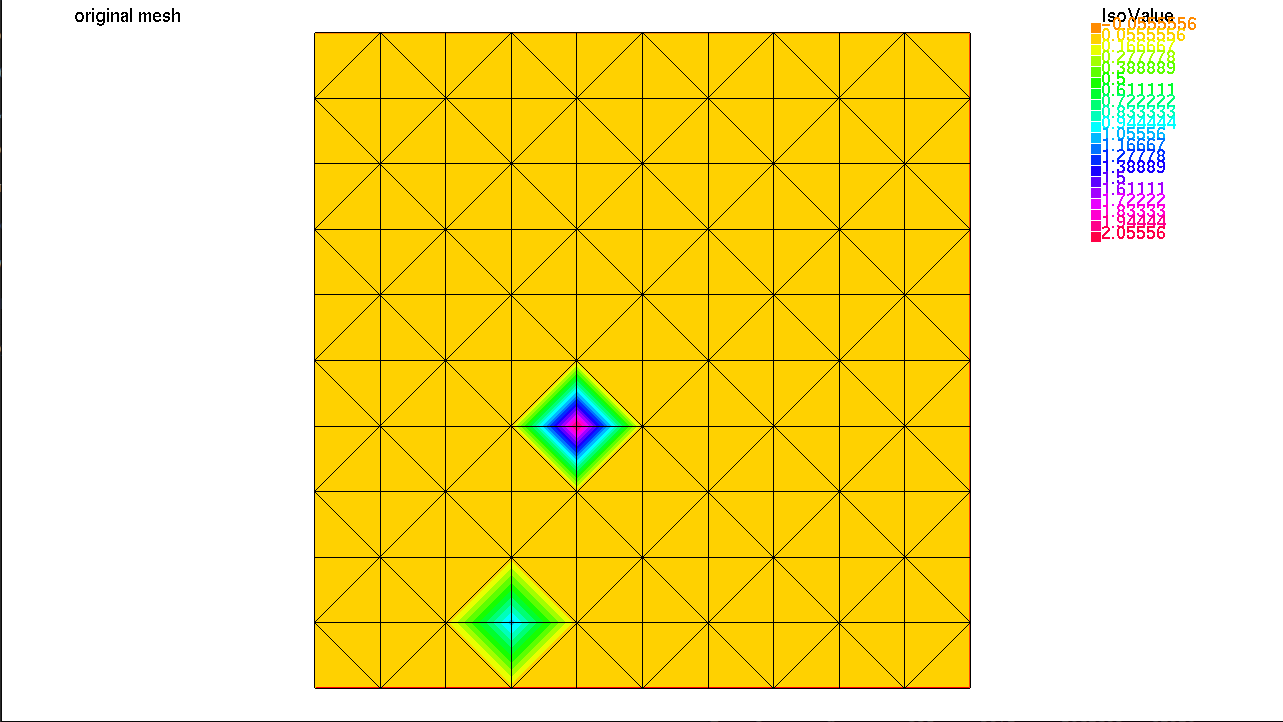
\includegraphics[width=0.7\linewidth]{img/origMesh.png}
	\caption{Исходная сетка и аппроксимация дельта-функции}
	\label{fig:Original}
\end{figure}
В приведенном примере кода дельта-функция задана в двух точках $xx = [.3, .4], yy = [.1, .4]$.
На рисунке \ref{fig:Original} видно, что значения "точечных" функций не превышают
заданных в коде значений $dd = [1, 2]$, причем сами функции равны нулю во всех узлах кроме
отдельных точек $xx = [.3, .4], yy = [.1, .4]$.
Аналогично, на рисунке \ref{fig:Split} максимальные значения функций по-прежнему не превышают
$dd = [1, 2]$, однако носитель функции значительно меньше по площади, чем на рисунке \ref{fig:Original}.
Очевидно, что и решения будут отличаться для двух сеток, а критерием остановки для адаптации сетки будет 
выполнение условия \refeq{eq:well_flowrate} 
\begin{figure}[H]
	\centering
	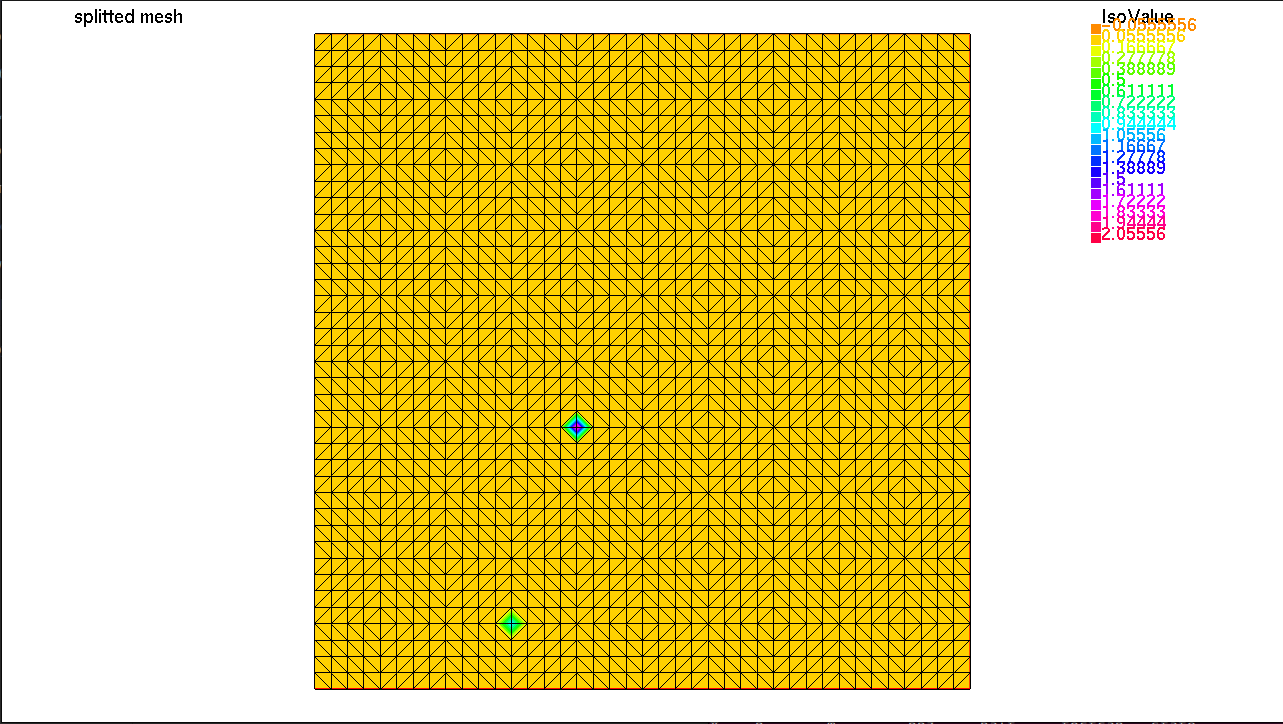
\includegraphics[width=0.7\linewidth]{img/splitMesh.png}
	\caption{Адаптивная сетка и аппроксимация дельта-функции}
	\label{fig:Split}
\end{figure}
Следует отметить, что, например, решение уравнения Пуассона с дельта-функцией в правой части имеет 
особенность в точке задания расхода (\cite{Hunt} стр.29), а значит нужно в ходе решения изменять это 
давление в узлах внутри скважины, либо с помощью МШФ корректировать водонасыщенность узлов, попадающих 
в скважину.\\
Полный код для решения поставленной задачи приведен в разделе \ref{appendix:App1}, полученные результаты расчета в 
\ref{appendix:App2}.

\newpage
\begin{appendices}
	\section{Исходный код}\label{appendix:App1}
	Я тут пишу {\Huge large} буквами
	\newpage
	\section{Результаты расчета}\label{appendix:App2}
		Чё-то тута
	\end{appendices}

\newpage
\bibliography{bibbase_local.bib}
\bibliographystyle{plain}
\end{document}
